
% Prepared by Calvin Kent
%
% Assignment Template v19.02
%
%%% 20xx0x/MATHxxx/Crowdmark/Ax
%
\documentclass[12pt]{article} %
\usepackage{CKpreamble}
\usepackage{CKassignment}
\usepackage{tkz-euclide}
\usepackage{physunits}
\usepackage{physics}
\usepackage{mathtools}
\usepackage{lmodern}

\usepackage{pgfplots}
\usepgfplotslibrary{polar}
\usepgflibrary{shapes.geometric}
\usetikzlibrary{calc}


\usepackage{euscript}
\usepackage{microtype}
\usepackage{upgreek}
\usepackage[misc]{ifsym}


%%Title
\title{\textbf{Assignment 2 Functions} \\ \textbf{Due Date: } Wednesday, January 19}
\date{January, 2022}

%%% Maths and science packages

\usepackage{amsmath,amsthm,amssymb}
\usepackage{pgfplots}
	\usetikzlibrary{
		calc,
		patterns,
		positioning
	}
	\pgfplotsset{
		compat=1.16,
		samples=200,
		clip=false,
		my axis style/.style={
			axis x line=middle,
			axis y line=middle,
			legend pos=outer north east,
			axis line style={
				->,
			},
			legend style={
				font=\footnotesize
			},
			label style={
				font=\footnotesize
			},
			tick label style={
				font=\footnotesize
			},
			xlabel style={
				at={
					(ticklabel* cs:1)
				},
				anchor=west,
				font=\footnotesize,
			},
			ylabel style={
				at={
					(ticklabel* cs:1)
				},
				anchor=west,
				font=\footnotesize,
			},
			xlabel= $x$,
			ylabel=$\vec d (\m \tx{[East]})$
		},
	}
	\tikzset{
		>=stealth
	}

\pgfplotsset{my style/.append style={axis x line=middle, axis y line=
middle, xlabel={$t$}, ylabel={$y[\text{m}]$}, axis equal }}

%%% Tables and figures packages

\usepackage{float}
\usepackage{caption}
	\captionsetup{
		format=plain,
		labelfont=bf,
		font=small,
		justification=centering
	}
	
%%% Numbers and sets

\newcommand{\E}{\mathrm{e}}

\newcommand{\tx}[1]{\text{#1}}
\newcommand{\rem}[1]{\operatorname{rem}{(#1)}}


%
\begin{document}
	\pagenumbering{arabic}
	% Start of class settings ...
	\renewcommand*{\coursecode}{MATH 235} % renew course code
	\renewcommand*{\assgnnumber}{Assignment 1} % renew assignment number
	\renewcommand*{\submdate}{September 14, 2021} % renew the date
	\renewcommand*{\studentfname}{Abdullah} % Student first name
	\renewcommand*{\studentlname}{Zubair} % Student last name
    \renewcommand*{\proofname}{Proof:}
	% \renewcommand*{\studentnum}{20836288} % Student number

	\renewcommand\qedsymbol{$\blacksquare$}
	\setfigpath
	% End of class settings	
	% \pagestyle{crowdmark}
	\newgeometry{left=18mm, right=18mm, top=22mm, bottom=22mm} % page is set to default values
	\fancyhfoffset[L,O]{0pt} % header orientation fixed
	% End of class settings
	%%% Note to user:
	% CTRL + F <CHANGE ME:> (without the angular brackets) in CKpreamble to specify graphics paths accordingly.
	% The command \circled[]{} accepts one optional and one mandatory argument.
	% Optional argument is for the size of the circle and mandatory argument is for its contents.
	% \circled{A} produces circled A, with size drawn for letter A. \circled[TT]{A} produces circled A with size drawn for TT.
	% https://github.com/CalvinKent/My-LaTeX
	%%%

	%%%%%%%%%%%%%%%%%%%%%%%%%%%%%%%%%%%%%%%%%%%%%%%%%%%%%%%%%%%%%%%%%%%%%%%%%%%%%%%
	%%%                        CUSTOM MACRO VIM-TEX                             %%%
	%%       call IMAP('NOM', '\nomenclature{}', 'tex')               

	%%%%%%%%%%%%%%%%%%%%%%%%%%%%%%%%%%%%%%%%%%%%%%%%%%%%%%%%%%%%%%%%%%%%%%%%%%%%%%%

	% Crowdmark assignment start
	% qnumber, qname, qpoints
\maketitle
	\section{Preamble}
  This assignment covers everything taught so far. The solutions that you hand in should be \textbf{neat} and \textbf{legible},
  this is an assignment, not a quiz, so I expect you to take your time and present thorough and detailed solutions.
\section{Name and Date:}
	Print your name and todays date below;\\


	\begin{center}
	\noindent\begin{tabular}{ll}
		\makebox[3in]{\hrulefill} & \makebox[3in]{\hrulefill}\\
		Name & Date\\[8ex]% adds space between the two sets of signatures
	\end{tabular}
	\end{center}
	\newpage



\begin{qstn}
  There exists a function that allows us to determine the length of a binary string.\\We call
  this function $\operatorname{len}$. Here a few examples to understand how it works,
  \begin{itemize}
    \item If $\textbf{S} = 1001$, then $\operatorname{len}(\textbf{S}) = 4$.
    \item If $\textbf{R} = 110001$, then $\operatorname{len}(\textbf{R}) = 6$.
    \item If $\textbf{T} = \epsilon$, then $\operatorname{len}(\textbf{T}) = 0$.
  \end{itemize}

  We can also define the operation of $ \textit{multiplication by a scalar}$ for binary strings. So suppose $n \in
  \mathbb N$ and \textbf{S} is some binary string, then,
    \[
      n\cdot \textbf{S} = \underbrace{\textbf{S} + \dots + \textbf{S}}_{\text{n times}}
    \]
  Again we resort to a few examples to demonstrate how multiplication by a scalar works,
  \begin{itemize}
    \item If $\textbf{S} = 1001$,  then $2\cdot\textbf{S} = \textbf{S} + \textbf{S} = 10011001$.
    \item If $\textbf{R} = 0$,  then $4\cdot\textbf{R} = \textbf{R} + \textbf{R} + \textbf{R} + \textbf{R} = 0000$.
    \item If $\textbf{T} = 01$,  then $3\cdot\textbf{T} = \textbf{T} + \textbf{T} + \textbf{T} = 010101$.
  \end{itemize}
  
Let $\textbf{S} = 001$ and $\textbf{T} = 11$, answer the following,
  \begin{enumerate}[label=(\alph*)]
    \item Let $\mathbb S$ represent the set of all binary strings. Define the length function using mapping
      notation.
    \item Compute $ \operatorname{len}(\textbf{S})$.
    \item Compute $ \operatorname{len}(\textbf{T})$.
    \item Compute $ \operatorname{len}(\textbf{S + T})$.
    \item Compute $ \operatorname{len}(3\cdot\textbf{S})$.
    \item Compute $ 3\cdot \operatorname{len}(\textbf{S})$.
    \item Compute $ \operatorname{len}(4\cdot\textbf{T})$.
    \item Compute $ 4\cdot \operatorname{len}(\textbf{T})$.
  \end{enumerate}

\begin{qstn}
  Let $F$ be a function. We call $F$ linear if both of the following conditions are satisfied,
  \begin{enumerate}
    \item For all inputs $x$ and $y$, 
      \[
          F(x+y) = F(x) + F(y)
      .\] 
    \item For all $c \in \mathbb F$, and all inputs $x$,
       \[
          F(c\cdot x) = c\cdot F(x)
      .\] 
  If $\mathbb F = \mathbb N$, then based on your results from Question 1, do you think that the length function, 
  $ \operatorname{len}$, is linear?
  Explain your answer.
  \end{enumerate}

\end{qstn}

\newpage

\begin{qstn}
  Sometimes in math we would like a function that simply gets rid of trailing decimals and returns a whole number,
  aka an integer. This function is known as the floor function. We define it with mapping notation as $ \operatorname{floor} \colon
  \R \to \Z$, and it works as follows, if $x \in \R$, then $\operatorname{floor}(x)$ is the
  smallest integer that is less than or equal to $x$.
  Lets see how it works in the following examples,
  \begin{itemize}
    \item If $x = 4.2$, then $\operatorname{floor}(x) = \operatorname{floor}(4.2) =  4$.
    \item If $x = -7.4$, then $\operatorname{floor}(x) = \operatorname{floor}(-7.4) = -8$.
    \item If $x = 5$, then $\operatorname{floor}(x) = \operatorname{floor}(5) =  5$.
    \item If $x = 0.4$, then $\operatorname{floor}(x) = \operatorname{floor}(0.4) =  0$.
  \end{itemize}
\end{qstn}
\begin{enumerate}[label=(\alph*)]
  \item Compute $ \operatorname{floor}(2.5)$.
  \item Compute $ \operatorname{floor}(6 / 3)$.
  \item Compute $ \operatorname{floor}(19 / 4)$.
  \item Let $f(x) = (x + 1) / 2$ and $g(x) = \sqrt{x - 1}$, compute $ \operatorname{floor}(f(g(5))$.
  \item Is the floor function linear? If it is, then justify your claim. If it is not, then provide a counter example to
        show that it fails to be linear.
  \item Is the floor function invertible? If it is, then justify your claim. If it is not, then provide a counter example to
        show that it fails to be surjective or injective. 
\end{enumerate}


\begin{qstn}
  Let $\EuScript{S} = \{1,010,00100,0001000\}$, where each element is a binary string, and let $\EuScript{R} =
  \{4,2,6,8\}$, where each element is a natural number.
  \begin{enumerate}[label=(\alph*)]
    \item Come up with an invertible function $\Psi$ between $\EuScript{S}$ and $\EuScript{R}$ and prove that your
      function is invertible. (\textbf{Hint:} Try using the length function)
    \item Come up with the correct formula for the inverse function $\Psi^{-1}$ and prove that your formula is
      correct using mapping tables. (\textbf{Hint:} The correct formula uses the floor function)
  \end{enumerate}
\end{qstn}

\begin{qstn}
  If you have ever kicked a soccer ball, you will have probably noticed that its trajectory closely imitates that
  of a parabola. This happens to be true under what we call ideal conditions, or in other words when the
  environment in which we kick the soccer ball is a vacuum. The primary motive behind this relationship is that
  gravitational acceleration does not effect motion in the horizontal direction, you'll learn more about this if
  you take a physics course. In this problem, we'll attempt to model different scenarios using transformations of
  functions. 

  Suppose I kick a ball from ground level at $t = 0$ seconds, I can model its trajectory as,

\begin{center}
\begin{tikzpicture}
  \begin{axis}[my style, minor tick num=1]

    \addplot[domain=0:4]{-(x -  2)^2 + 4};
    \node[label={45:{\textcolor{black}{$(2,4)$}}},circle,fill,inner sep=2pt] at (axis cs:2,4) {};
  \end{axis}
\end{tikzpicture}
\end{center}

We plot the time elapsed on the x-axis, and the height of the ball (in meters) on the y-axis. From the
figure above we see that at $t = 2$ seconds, the ball reached a height of $4$ meters.

\begin{enumerate}[label=(\alph*)]
  \item[(A)] We can model the equation of the trajectory as a transformation of $f(t) = -t^2$, 
        \[
              h(t) = f(t + A) + B
        .\] 
        \begin{enumerate}[label=(\alph*)]
          \item What are the correct values for $A$ and $B$?
          \item Determine the height of the ball at $t = 3$ seconds.
          \item Determine the height of the ball at $t = 4$ seconds.
          \item Determine the height of the ball at $t = 1$ seconds.
        \end{enumerate}
  \item[(B)] I kick the ball a second time, this time not as high, and get the following trajectory (Graph
    indicated with arrow),
      \begin{center}
          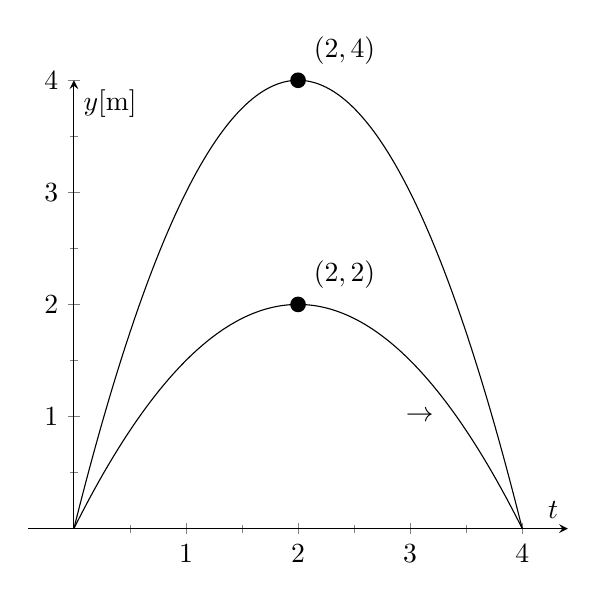
\begin{tikzpicture}
            \begin{axis}[my style,  minor tick num=1]

              \addplot[domain=0:4]{-(x -  2)^2 + 4};
              \addplot[domain=0:4]{0.5*(-(x -  2)^2 + 4)};

              \node[label={45:{\textcolor{black}{$(2,4)$}}},circle,fill,inner sep=2pt] at (axis cs:2,4) {};
              \node[label={45:{\textcolor{black}{$(2,2)$}}},circle,fill,inner sep=2pt] at (axis cs:2,2) {};
              \node[label={0:{\textcolor{black}{$\rightarrow$}}},circle,inner sep=2pt] at (axis cs:2.8,1) {};
            \end{axis}
          \end{tikzpicture}
      \end{center}
      \newpage
      We can model the equation of the trajectory as a vertical scaling of $h(t)$, 
        \[
              g(t) = K\cdot h(t)
        .\] 
    \begin{enumerate}[label=(\alph*)]
      \item What is the correct value for $K$? Also describe the precise vertical scaling that occurred.
      \item What was the height of the ball at $t = 1$ seconds?
      \item What was the height of the ball at $t = 3$ seconds?
      \item What was the height of the ball at $t = 4$ seconds?
    \end{enumerate}


  \item[(C)] I then told my sister to kick the ball, and modelled her trajectory as (Graph
    indicated with arrow),
      \begin{center}
          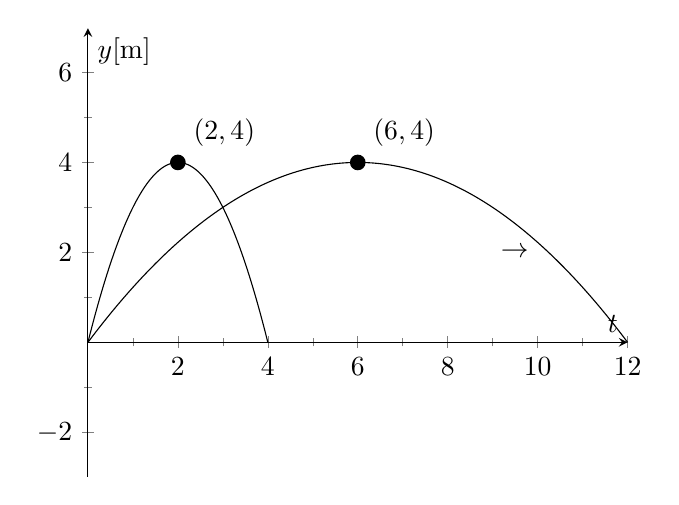
\begin{tikzpicture}
            \begin{axis}[my style, minor tick num=1]

              \addplot[domain=0:4]{-(x -  2)^2 + 4};
              \addplot[domain=0:12]{-(0.3333333*x -  2)^2 + 4};

              \node[label={45:{\textcolor{black}{$(2,4)$}}},circle,fill,inner sep=2pt] at (axis cs:2,4) {};
              \node[label={45:{\textcolor{black}{$(6,4)$}}},circle,fill,inner sep=2pt] at (axis cs:6,4) {};
              \node[label={180:{\textcolor{black}{$\rightarrow$}}},circle,inner sep=2pt] at (axis cs:10.2,2) {};
            \end{axis}
          \end{tikzpicture}
      \end{center}
      We can model the equation of her trajectory as a horizontal scaling of $h(t)$, 
        \[
              s(t) = h(D\cdot t)
        .\]
      \begin{enumerate}[label=(\alph*)]
        \item What is the correct value for $D$? Also describe the precise horizontal scaling that occurred.
        \item What was the height of the ball at $t = 3$ seconds?
        \item What was the height of the ball at $t = 9$ seconds?
        \item What was the height of the ball at $t = 12$ seconds?
        \item Based on her trajectory, did the ball travel farther horizontally for her kick? Explain your
          answer.

      \end{enumerate}


\end{enumerate}



  
\end{qstn}














\end{qstn}













\end{document}



































